\documentclass{article}

% if you need to pass options to natbib, use, e.g.:
\PassOptionsToPackage{numbers, compress}{natbib}
% before loading neurips_2021

% ready for submission
% \usepackage{neurips_2021}

% to compile a preprint version, e.g., for submission to arXiv, add add the
% [preprint] option:
\usepackage[preprint]{neurips_2021}

% to compile a camera-ready version, add the [final] option, e.g.:
%     \usepackage[final]{neurips_2021}

% to avoid loading the natbib package, add option nonatbib:
%    \usepackage[nonatbib]{neurips_2021}

\usepackage[utf8]{inputenc} % allow utf-8 input
\usepackage[T1]{fontenc}    % use 8-bit T1 fonts
\usepackage{hyperref}       % hyperlinks
\usepackage{url}            % simple URL typesetting
\usepackage{booktabs}       % professional-quality tables
\usepackage{amsfonts}       % blackboard math symbols
\usepackage{nicefrac}       % compact symbols for 1/2, etc.
\usepackage{microtype}      % microtypography
\usepackage{xcolor}         % colors
\usepackage{graphicx}
\usepackage{subfigure}

\title{Digital recognization by five methods}

% The \author macro works with any number of authors. There are two commands
% used to separate the names and addresses of multiple authors: \And and \AND.
%
% Using \And between authors leaves it to LaTeX to determine where to break the
% lines. Using \AND forces a line break at that point. So, if LaTeX puts 3 of 4
% authors names on the first line, and the last on the second line, try using
% \AND instead of \And before the third author name.

\author{
	Lanhe Gao 2018533212\\
	SIST\\
	ShanghaiTech University\\
	Shanghai, China \\
	\texttt{gaolh@shanghaitech.edu.cn} \\
	\And
	Yunfei Zhang 2018533098\\
	SIST\\
	ShanghaiTech University\\
	Shanghai, China \\
	\texttt{zhanyf2@shanghaitech.edu.cn} \\
}

\begin{document}
	
	\maketitle
	
	\begin{abstract}
		Recognizing handwritten numbers is a very classical machine learning problem, which has a variety of solutions. In this report, we try to implement five of these methods. By comparing their performances, we hope to choose the best one.
	\end{abstract}

	\section{Introduction}
	
	Number recognization is a widely used application, with great sophistication. There are many types of machine learning methods that can be used in this scenario. In this report, we have adopted five methods, such as Support Vector Machine (SVM), K-Nearsest Neighbors (KNN), Naive Bayes (NB), Neural Networks (NN) and Logistic Regression (LR). We will analyze the accuracy, runtime performance, confusion matrix and other standards to compare their performance, and conclude the best method.
	
	\section{Data Setting and Methods}
	
	\subsection{Data setting}
	
	Our training data and testing data are collected from \textit{mnist} dataset. They're in the same form, with 28*28 pixels, therefore, we use a 784 dimensional vector to represent each number picture. The pictures are gray images, scaling from 0 to 255.
	
	\subsection{KNN}
	
	The first method we use is KNN. Consider that each picture is composed of 784 pixels. If we expand it into a 784-dimensional vector in a fixed spatial order, we can put each test point into a hyperplane. Since the dimension is quite big, which makes the complexity of calculating 2-norm quite big, so we use 1-norm instead. KNN calculates K nearest images that has the smalles 1-norm distance to a given test data, and labels it as the class that contains the most number of neighbors. 
	
	It takes at least $O(784)$ time to calculate the distance for every two pictures. The number of samples in the training set is 60,000, the number of samples in the test set is 10,000, and the time responsibility is $O(5*10^11)$, which is too long. In our test, we select the first 100 test set samples for testing, which approximates the matching rate of the KNN algorithm.
	
	The code implementation is at 
	\begin{center}
		\url{https://github.com/chuansao-258/machine-learning--digital-recognition/blob/main/knn.ipynb}
	\end{center}
	
	\subsection{SVM}
	
	The SVM algorithm was originally designed for binary classification problems. When dealing with multi-class problems, it is necessary to construct a suitable multi-class classifier. So when extracting the training set, take class $0$ as an example, extract:
	
	\begin{equation}
		+: 0, -: 1\sim 8
	\end{equation}

	Other class work similarly. When testing, use the ten training result files to test the corresponding test vectors. Finally, each test has a result $f_0(x), f_1(x), \cdots, f_{9}(x)$. The final result is the largest of these four values as the classification result.
	
	We use the svm from \textit{sklearn} package. We directly put the data and label into the model \textit{svm.fit()} for training, then use \textit{svm.predict()} to run prediction. The code implementation is at
	\begin{center}
		\url{https://github.com/chuansao-258/machine-learning--digital-recognition/blob/main/SVM.ipynb}
	\end{center}
	
	\subsection{NB}
	
	In Bayes model. we assume all features are independent effects of the label. Simple digit recognition version: One feature(variable) $F_{i, j}$ for each grid position $<i,j>$. Feature values are on/off, based on whether intensity is more or less than 0.5 in underlying image. Each input maps to a feature vector, e.g. Image1 $\rightarrow (F_{0, 0} = 0,  F_{0, 1}  = 0,  F_{0, 2}  = 1,..., F_{27, 27}  = 0)$. 
	
	 Then, the prediction works like this: given a test image, we calculate the probability multiplication of all pixel points, and choose the label with the highest probability, As shown in Figure \ref{bayes}.
	 
	 \begin{figure}[htbp]
	 	\centering
	 	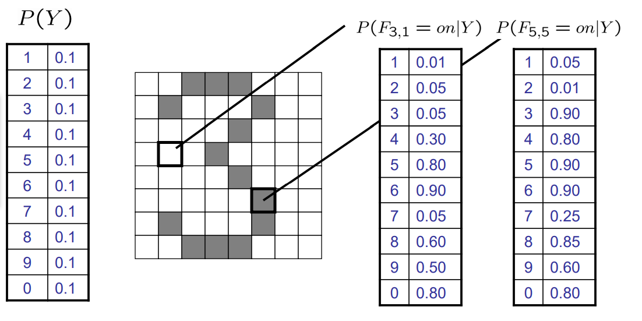
\includegraphics[scale=0.6]{1.png}
	 	\caption{Bayes classification}
	 	\label{bayes}
	 \end{figure}
	 
	 Before coding, we tried the naive bayes model in sklearn. However, it does not work well, with only 58\% accuracy, so we try to implement one by ourselves. The code implementation is at 
	 \begin{center}
	 	\url{https://github.com/chuansao-258/machine-learning--digital-recognition/blob/main/bayes.ipynb}
	 \end{center}
 	 
 	 \subsection{LR}
 	 
 	 Similar to SVM, Logistic Regression is also a binary classification method. However, we want to classify these handwritings into 10 classes, so we need to extend LR method as well. For each class, we devide the dataset into the ones belong to the class, and the ones do not. For example, from class $0$'s perspective, the dataset would be labeled as:
 	 
 	 \begin{equation}
 	 	+: 0, -: 1\sim 8
 	 \end{equation}
  
	This turns out to be a binary classification problem now, and we need to do it for every class, 10 times in total. Finally, we choose the class that the input has the highest probability on. 
	
	We use the LogisticRegression model in sklearn to implement this method. The code implementation is at
	
	\begin{center}
		\url{https://github.com/chuansao-258/machine-learning--digital-recognition/blob/main/Logistic\%20Regression.ipynb}
	\end{center}
 	 
 	 \subsection{NN}
 	 
	The settings of the neural network is displayed as Figure \ref{nn.1} and \ref{nn.2}. The first 784 layers enter the neural network as input. The 15th layer is used as the middle layer; after passing through the middle layer, it enters the activation function 10 layers as the output layer, representing the possible probability of each picture for each number. Choose the largest one as the prediction result, and use the gradient descent method to modify the values of m1, b1, m2, and b2.
	 
	 \begin{figure}[htbp]
	 	\centering
	 	\subfigure{
	 		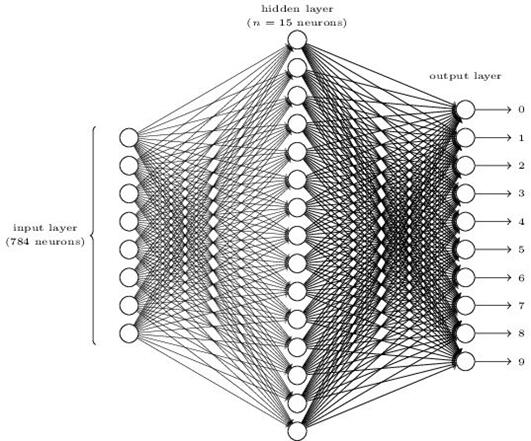
\includegraphics[scale=0.5]{4.png}
 			\label{nn.1}}
 		\subfigure{
 			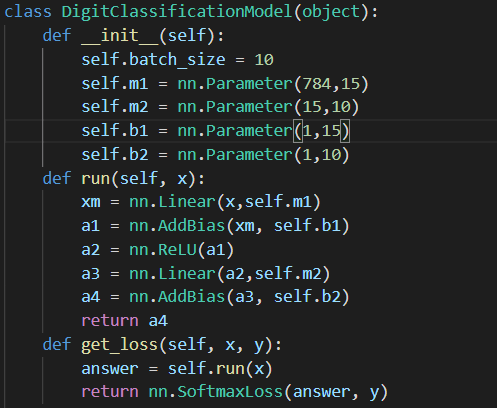
\includegraphics[scale=0.35]{3.png}
 			\label{nn.2}}
	 	\caption{Neural network setting}
	 \end{figure}
 
 	 The code implementation is at
 	
 	\begin{center}
 		\url{https://github.com/chuansao-258/machine-learning--digital-recognition/tree/main/nn}
 	\end{center} 
	 
	 \section{Performance}
	 
	 All the performances can be checked in the code implementation.
	 
	 \subsection{KNN}
	 
	 The parameters of KNN we set is: 
	 \begin{itemize}
	 	\item Manhattan distance
	 	\item k = 5
	 \end{itemize} 
 	And the accuracy is 47.00\%. This method takes long time to calculate and the performance is not good.
 	
 	\subsection{NB}
 	
 	To prevent the case that the probability might fall to 0, we set $0 = 1e^-7$. The accuracy is 68.41\%
 	
 	\subsection{LR}
 	
 	We set the solver in LogisticRegression model in sklearn as 'saga', and the accuracy is 92.57\%. This method can be seen as neural network without hidden layer, so we expect higher accuracy in NN method.
 	
 	\subsection{SVM}
 	
 	In the SVM model, there are two factors that might affect the accuracy,
 	\begin{itemize}
 		\item max\_iter: the number of iterations.
 		\item kernel: the kernel function type. the choices are 'linear', 'poly' and 'sigmoid'.
 	\end{itemize}
 	We've adjusted these two and the results are shown in Figure \ref{svm1} and \ref{svm2}.
 	
 	\begin{figure}[htbp]
 		\centering
 		\subfigure[accuracy-kernel]{
 			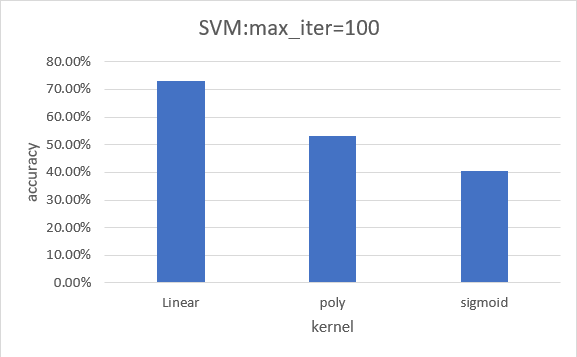
\includegraphics[scale=0.3]{per1.png}
 			\label{svm1}}
 		\subfigure[accuracy-max\_iter]{
 			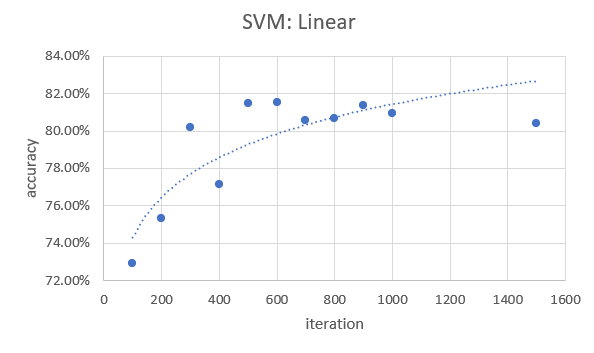
\includegraphics[scale=0.3]{per2.png}
 			\label{svm2}}
 		\caption{SVM performance of two factors}
 	\end{figure}
	
	We can see that linear kernel with high iteration number, the accuracy could be very high, about 82\%. 
	
	\subsection{NN}
	
	In NN model, we find three factors that might affect the accuacy,
	
	\begin{itemize}
		\item layer1: the number of units in the hidden layer. the choices are 15 or 100.
		\item batch\_size: the number of training samples to choose in each round of training. the choices are 10 and 100.
		\item iteration: the number of iterations in training.
	\end{itemize}

	We've compared six groups of parameters, and the performance is shown in Figure \ref{nn}. Apparently, the set $[100, 10, 30]$ works the best, with about 97.94\%
	
	\begin{figure}[htbp]
		\centering
		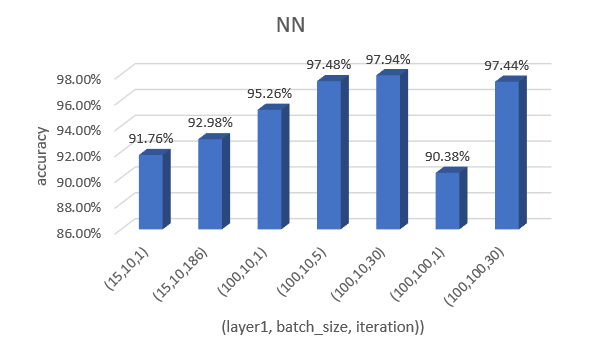
\includegraphics[scale=0.35]{per3.png}
		\caption{NN performance of three factors}
		\label{nn}
	\end{figure}

	\section{Conclusion}
	
	After impleenting these five methods, we can conclude that neural network works the best, with an astonishing 97.94\% accuracy. However, there are other choices, like convolutional neural network, recursive neural network, decision tree and so on. We hope to develop their possiblities in achieving higher accuracy in further research and implementation.
	
	%%%%%%%%%%%%%%%%%%%%%%%%%%%%%%%%%%%%%%%%%%%%%%%%%%%%%%%%%%%%
	
\end{document}